\chapter{Project}
\label{ch:project}

\section{Mapping Steering Mirror Coordinates to Target Plane Coordinates}
\label{sec:Mapping Steering Mirror Coordinates to Target Plane Coordinates}

To direct the laser beam MR-E-2 beam steering mirror is used.
Laser beam is produced by a laser which is stationary. Laser
is positioned to hit the steering mirror in the center. After
the beam hits the mirror, it is directed to required position
by adjusting the position of the mirror.


\begin{figure}[!htb]\centering
    \includegraphics*[width = 6cm]{bilder/project/setup.jpg}
    \caption{Laser, depth camera, and beam steering mirror setup}
    \label{fig:setup}
\end{figure}

Using the mirror to steer the laser beam requires a mapping from
3D world coordinate system to mirror coordinate system. The
mapping calculates the required rotation of the mirror around
its axes to direct the laser beam to intended 3D position.
Mirror coordinate system is defined in [1] as in following figure.




\begin{figure}[!htb]\centering
    \includegraphics*[width = 6cm]{bilder/project/mirror_coordinates.png}
    \caption{Internal mirror coordinate system[1]}
    \label{fig:mirror_coordinates}
\end{figure}


The coordinate system is a Cartesian coordinate system with X and Y axes.
Rotation of the mirror around its horizontal and vertical axes are expressed
as x and y values. The range of both axes are [-1, 1] interval. Mirror
has maximum deflection angle of 25\degree .  $\theta$ is the angle between
incoming and reflected beam.  $\theta$ = +50\degree  corresponds to +1
and $\theta$ = -50\degree  corresponds to -1.  X and Y values are required
to be inside a unit circle in order to be a valid point accessible by the mirror.



\begin{figure}[!htb]\centering
    \includegraphics*[width = 6cm]{bilder/project/mirror_rotation.png}
    \caption{Relation between rotation of the mirror ($\theta$) and the
    mirror coordinate (x) in X-axis[1]}
    \label{fig:mirror_rotation}
\end{figure}



\begin{figure}[!htb]\centering
    \includegraphics*[width = 12cm]{bilder/project/coordinate_systems.png}
    \caption{Mirror coordinate system [1]}
    \label{fig:coordinate_systems}
\end{figure}


In the system setup used in experiments following configuration is used:
\begin{itemize}
    \item $P_{1} = M = C$
    \item $O = P_{1} = M = C$
    \item $d = 0$
    \item Incoming ray is coming in y-z plane.
\end{itemize}


The conversion of coordinates on target plane $(x_{t}, y_{t})$ to mirror
coordinates $(x, y)$ is performed in two main steps. Firstly,
the mirror normal ($n_{m}$) is calculated based on position of the
laser, position of the target plane and $(x_{t}, y_{t})$. In the next
step, corresponding mirror coordinates $(x, y)$ is calculated using $n_{m}$.

\subsection{Computation of mirror normal vector $(n_{m})$}
\label{subsec:compute_mirror_normal}

There are 2 different frames of reference I and T. Reference
frame I is centered around $O$. Its z-axis is aligned with $-n_{m}$ direction
and its y-axis is aligned so that incoming laser beam propagates
through yz plane.  Reference frame T is centered around T.
Its z-axis is aligned with $n_{t}$ direction and its y-axis is aligned
so that reflected laser beam propagates through yz plane.
The transformation between frame of references is done with orthogonal
transformation matrices $A_{IT}$ and $A_{TI}$.



\begin{align*}
    n^{T}_{t}       & =
    \begin{bmatrix}
        0 \\
        0 \\
        1
    \end{bmatrix} &
    r^{T}_{OT}      & =
    \begin{bmatrix}
        0 \\
        0 \\
        -D
    \end{bmatrix}      \\
    r^{T}_{TP_{2}}  & =
    \begin{bmatrix}
        x_{t} \\
        y_{t} \\
        0
    \end{bmatrix} &
    n^{I}_{0}       & =
    \begin{bmatrix}
        0 \\
        0 \\
        1
    \end{bmatrix}      \\
    A_{IT}          & =
    \begin{bmatrix}
        1 & 0           & 0            \\
        0 & cos(\alpha) & -sin(\alpha) \\
        0 & sin(\alpha) & cos(\alpha)
    \end{bmatrix}
\end{align*}


Mirror normal vector is calculated with following steps:

\begin{align*}
    n^{I}_{t}      & = A_{IT} \cdot n^{T}_{t}          \\
    n^{I}_{OT}     & = A_{IT} \cdot r^{T}_{OT}         \\
    r^{I}_{TP_{2}} & = A_{IT} \cdot r^{T}_{TP_{2}}     \\
    r^{I}_{OP_{2}} & = r^{T}_{OT} \cdot r^{I}_{TP_{2}} \\
    n^{I}_{1}      & = normalize(r^{I}_{OP_{2}})       \\
    n^{I}_{m}      & = normalize(n_{1} - n_{0})
\end{align*}

\subsection{Computation of mirror coordinates $(x, y)$ }
\label{subsec:compute_mirror_coordinates}


\begin{align*}
    r^{I}_{C}       & =
    \begin{bmatrix}
        0 \\
        0 \\
        d
    \end{bmatrix} &
    N^{I}_{0}       & =
    \begin{bmatrix}
        0 \\
        0 \\
        -1
    \end{bmatrix}      \\
    n^{T}_{t}       & =
    \begin{bmatrix}
        0 \\
        0 \\
        1
    \end{bmatrix} &
    r^{T}_{OT}      & =
    \begin{bmatrix}
        0 \\
        0 \\
        -D
    \end{bmatrix}      \\
    A_{IT}          & =
    \begin{bmatrix}
        1 & 0 & 0 \\
        0 & 1 & 0 \\
        0 & 0 & 1
    \end{bmatrix}
\end{align*}




\begin{align*}
    t_{1}          & = \frac{ (R^{I}_{C} - r^{I}_{OP_{0}}) \cdot n^{I}_{m} + d }{n^{I}_{0} \cdot n^{I}_{m}} \\
    r^{I}_{OP_{1}} & = r^{I}_{OP_{0}} + t_{1} \cdot n^{I}_{0}                                               \\
    n^{I}_{1}      & = n^{I}_{0} - 2 \cdot ( n^{I}_{0} \cdot n^{I}_{m}) \cdot n^{I}_{m}                     \\
    t_{2}          & = \frac{ (r^{T}_{OT} - r^{I}_{OP_{1}}) \cdot n^{T}_{t}}{n^{I}_{1} \cdot n^{T}_{t}}     \\
    r^{I}_{OP_{2}} & = r^{I}_{OP_{1}} + t_{2} \cdot n^{I}_{1}                                               \\
    x              & = \frac{ r^{I}_{OP_{2}}[0] }{D \cdot tan(50 \degree)}                                  \\
    y              & = \frac{ r^{I}_{OP_{2}}[1] }{D \cdot tan(50 \degree)}
\end{align*}




\section{Position Error Measurement System}
\label{sec:Position Error Measurement System}





\begin{figure}[!htb]\centering
    \includegraphics*[width = 10cm]{bilder/project/error_test_setup.jpg}
    \caption{Position error test setup}
    \label{fig:error_test}
\end{figure}

Measurements are done with a 2-dimensional servo motor system with
a PM400 power meter attached.
Measurements are performed by pointing the laser to a specified
target position and then sweeping the power meter in a linear
trajectory. Power recordings are recorded with recording times
and plotted to find the instance with maximum power. The point
with maximum power gives the center position of the laser.
Power measurements are performed by a Python script which
has a loop with a period of around 0.01s. This sampling
period is not constant throughout the measurements and
might deviate from 0.01s.  For this reason, after the
measurement, cubic interpolation is performed to get
a uniformly sampled signal.


\begin{figure}[!htb]\centering
    \includegraphics*[width = 16cm]{bilder/project/error_test_graph_1.png}
    \caption{Power(mW) - Position(mm) graphs for raw signal and cubic interpolation signal}
    \label{fig:error_test_graph_1}
\end{figure}


Interpolation solves the nonuniform sampling problem.
Obtained signal still has noise in it which might alter
the maximum position. To remove the noise a low pass
filter in the form of a moving average filter is applied.
The figure below depicts the signal before and after the
low pass filter. High-frequency noise components are
removed from the signal while keeping the original signal
mostly intact. This operation produced a smoother signal
which is more suitable for peak finding operation.


\begin{figure}[!htb]\centering
    \includegraphics*[width = 16cm]{bilder/project/error_test_graph_2.png}
    \caption{Power(mW) - Position(mm) graphs for raw signal and cubic interpolation signal}
    \label{fig:error_test_graph_2}
\end{figure}


The recorded power signal is plotted with respect to distance
in order to find the position of the laser's center. This method
gives the position of the laser relative to the initial position
of the servo motor. The figure below shows the power levels with
respect to time and position. Position with maximum power is written
in the fourth graph in millimeters.


\begin{figure}[!htb]\centering
    \includegraphics*[width = 16cm]{bilder/project/error_test_graph_3.png}
    \caption{Power(mW) - Position(mm) graphs for raw signal and cubic interpolation signal}
    \label{fig:error_test_graph_3}
\end{figure}


Measurements are performed with different parameters such as the distance
between the mirror and target plane, different sweep locations.


\subsection{Test results }
\label{subsec:test_results}

The coordinate systems that are used in the steering
mirror and the depth camera don't coincide. They are
rotated and translated versions of each other. A point
in camera coordinate system, c, can be transformed into
a point in mirror coordinate system, m, with the following mapping:


\begin{table}[ht]
    \captionabove{Distance between mirror and target plane is set to 410mm. Actual distance between mirror and target plane is 425mm.} %%%%%%%%%%%%%%%%%%%%%%%%%%%%
    \centering
    \begin{tabular}{| c | c | c | c |} %Ausrichtung festlegen
        \hline Mirror Input x & Mirror Input y & Peak Power Position & Relative Distance \\ \hline % Überschriften
        \SI{-3}{mm}           & \SI{-5}{mm}    & \SI{2.322}{mm}      & \SI{-3.096}{mm}   \\
        \SI{-2.5}{mm}         & \SI{-5}{mm}    & \SI{2.853}{mm}      & \SI{-2.565}{mm}   \\
        \SI{-2}{mm}           & \SI{-5}{mm}    & \SI{3.372}{mm}      & \SI{-2.046}{mm}   \\
        \SI{-1.5}{mm}         & \SI{-5}{mm}    & \SI{3.868}{mm}      & \SI{-1.550}{mm}   \\
        \SI{-1}{mm}           & \SI{-5}{mm}    & \SI{4.392}{mm}      & \SI{-1.026}{mm}   \\
        \SI{-0.5}{mm}         & \SI{-5}{mm}    & \SI{4.905}{mm}      & \SI{-0.513}{mm}   \\
        \SI{0}{mm}            & \SI{-5}{mm}    & \SI{5.418}{mm}      & \SI{0}{mm}        \\
        \SI{0.5}{mm}          & \SI{-5}{mm}    & \SI{5.921}{mm}      & \SI{0.503}{mm}    \\
        \SI{1}{mm}            & \SI{-5}{mm}    & \SI{6.446}{mm}      & \SI{1.028}{mm}    \\
        \SI{1.5}{mm}          & \SI{-5}{mm}    & \SI{6.923}{mm}      & \SI{1.505}{mm}    \\
        \SI{2}{mm}            & \SI{-5}{mm}    & \SI{7.427}{mm}      & \SI{2.009}{mm}    \\
        \SI{2.5}{mm}          & \SI{-5}{mm}    & \SI{7.937}{mm}      & \SI{2.519}{mm}    \\
        \SI{3}{mm}            & \SI{-5}{mm}    & \SI{8.452}{mm}      & \SI{3.034}{mm}    \\

        \hline


        \SI{-3}{mm}           & \SI{0}{mm}     & \SI{2.278}{mm}      & \SI{-3.089}{mm}   \\
        \SI{-2.5}{mm}         & \SI{0}{mm}     & \SI{2.792}{mm}      & \SI{-2.575}{mm}   \\
        \SI{-2}{mm}           & \SI{0}{mm}     & \SI{3.311}{mm}      & \SI{-2.056}{mm}   \\
        \SI{-1.5}{mm}         & \SI{0}{mm}     & \SI{3.829}{mm}      & \SI{-1.538}{mm}   \\
        \SI{-1}{mm}           & \SI{0}{mm}     & \SI{4.327}{mm}      & \SI{-1.040}{mm}   \\
        \SI{-0.5}{mm}         & \SI{0}{mm}     & \SI{4.860}{mm}      & \SI{-0.507}{mm}   \\
        \SI{0}{mm}            & \SI{0}{mm}     & \SI{5.367}{mm}      & \SI{0}{mm}        \\
        \SI{0.5}{mm}          & \SI{0}{mm}     & \SI{5.878}{mm}      & \SI{0.511}{mm}    \\
        \SI{1}{mm}            & \SI{0}{mm}     & \SI{6.379}{mm}      & \SI{1.012}{mm}    \\
        \SI{1.5}{mm}          & \SI{0}{mm}     & \SI{6.880}{mm}      & \SI{1.513}{mm}    \\
        \SI{2}{mm}            & \SI{0}{mm}     & \SI{7.392}{mm}      & \SI{2.025}{mm}    \\
        \SI{2.5}{mm}          & \SI{0}{mm}     & \SI{7.880}{mm}      & \SI{2.513}{mm}    \\
        \SI{3}{mm}            & \SI{0}{mm}     & \SI{8.390}{mm}      & \SI{3.023}{mm}    \\

        \hline


        \SI{-3}{mm}           & \SI{5}{mm}     & \SI{2.391}{mm}      & \SI{-3.097}{mm}   \\
        \SI{-2.5}{mm}         & \SI{5}{mm}     & \SI{2.909}{mm}      & \SI{-2.579}{mm}   \\
        \SI{-2}{mm}           & \SI{5}{mm}     & \SI{3.424}{mm}      & \SI{-2.064}{mm}   \\
        \SI{-1.5}{mm}         & \SI{5}{mm}     & \SI{3.949}{mm}      & \SI{-1.539}{mm}   \\
        \SI{-1}{mm}           & \SI{5}{mm}     & \SI{4.468}{mm}      & \SI{-1.020}{mm}   \\
        \SI{-0.5}{mm}         & \SI{5}{mm}     & \SI{4.974}{mm}      & \SI{-0.514}{mm}   \\
        \SI{0}{mm}            & \SI{5}{mm}     & \SI{5.488}{mm}      & \SI{0}{mm}        \\
        \SI{0.5}{mm}          & \SI{5}{mm}     & \SI{6.013}{mm}      & \SI{0.525}{mm}    \\
        \SI{1}{mm}            & \SI{5}{mm}     & \SI{6.534}{mm}      & \SI{1.046}{mm}    \\
        \SI{1.5}{mm}          & \SI{5}{mm}     & \SI{7.042}{mm}      & \SI{1.554}{mm}    \\
        \SI{2}{mm}            & \SI{5}{mm}     & \SI{7.547}{mm}      & \SI{2.059}{mm}    \\
        \SI{2.5}{mm}          & \SI{5}{mm}     & \SI{8.052}{mm}      & \SI{2.564}{mm}    \\
        \SI{3}{mm}            & \SI{5}{mm}     & \SI{8.561}{mm}      & \SI{3.073}{mm}    \\
        \hline
    \end{tabular}
    %		\caption{Amateurfunkbänder (Auswahl)}
    \label{tab:d410}
\end{table}



\begin{table}[ht]
    \captionabove{Distance between mirror and target plane is set to 425mm. Actual distance between mirror and target plane is 425mm.} %%%%%%%%%%%%%%%%%%%%%%%%%%%%
    \centering
    \begin{tabular}{| c | c | c | c |} %Ausrichtung festlegen
        \hline Mirror Input x & Mirror Input y & Peak Power Position & Relative Distance \\ \hline % Überschriften
        \SI{-3}{mm}           & \SI{-5}{mm}    & \SI{6.723}{mm}      & \SI{-2.999}{mm}   \\
        \SI{-2.5}{mm}         & \SI{-5}{mm}    & \SI{7.225}{mm}      & \SI{-2.497}{mm}   \\
        \SI{-2}{mm}           & \SI{-5}{mm}    & \SI{7.727}{mm}      & \SI{-1.995}{mm}   \\
        \SI{-1.5}{mm}         & \SI{-5}{mm}    & \SI{8.218}{mm}      & \SI{-1.504}{mm}   \\
        \SI{-1}{mm}           & \SI{-5}{mm}    & \SI{8.716}{mm}      & \SI{-1.007}{mm}   \\
        \SI{-0.5}{mm}         & \SI{-5}{mm}    & \SI{9.228}{mm}      & \SI{-0.494}{mm}   \\
        \SI{0}{mm}            & \SI{-5}{mm}    & \SI{9.722}{mm}      & \SI{0.0}{mm}      \\
        \SI{0.5}{mm}          & \SI{-5}{mm}    & \SI{10.212}{mm}     & \SI{0.49}{mm}     \\
        \SI{1}{mm}            & \SI{-5}{mm}    & \SI{10.695}{mm}     & \SI{0.973}{mm}    \\
        \SI{1.5}{mm}          & \SI{-5}{mm}    & \SI{11.191}{mm}     & \SI{1.469}{mm}    \\
        \SI{2}{mm}            & \SI{-5}{mm}    & \SI{11.673}{mm}     & \SI{1.951}{mm}    \\
        \SI{2.5}{mm}          & \SI{-5}{mm}    & \SI{12.151}{mm}     & \SI{2.429}{mm}    \\
        \SI{3}{mm}            & \SI{-5}{mm}    & \SI{12.653}{mm}     & \SI{2.931}{mm}    \\

        \hline


        \SI{-3}{mm}           & \SI{0}{mm}     & \SI{6.788}{mm}      & \SI{-2.956}{mm}   \\
        \SI{-2.5}{mm}         & \SI{0}{mm}     & \SI{7.275}{mm}      & \SI{-2.469}{mm}   \\
        \SI{-2}{mm}           & \SI{0}{mm}     & \SI{7.777}{mm}      & \SI{-1.967}{mm}   \\
        \SI{-1.5}{mm}         & \SI{0}{mm}     & \SI{8.289}{mm}      & \SI{-1.455}{mm}   \\
        \SI{-1}{mm}           & \SI{0}{mm}     & \SI{8.758}{mm}      & \SI{-0.986}{mm}   \\
        \SI{-0.5}{mm}         & \SI{0}{mm}     & \SI{9.248}{mm}      & \SI{-0.496}{mm}   \\
        \SI{0}{mm}            & \SI{0}{mm}     & \SI{9.744}{mm}      & \SI{0.0}{mm}      \\
        \SI{0.5}{mm}          & \SI{0}{mm}     & \SI{10.225}{mm}     & \SI{0.481}{mm}    \\
        \SI{1}{mm}            & \SI{0}{mm}     & \SI{10.711}{mm}     & \SI{0.967}{mm}    \\
        \SI{1.5}{mm}          & \SI{0}{mm}     & \SI{11.207}{mm}     & \SI{1.463}{mm}    \\
        \SI{2}{mm}            & \SI{0}{mm}     & \SI{11.666}{mm}     & \SI{1.922}{mm}    \\
        \SI{2.5}{mm}          & \SI{0}{mm}     & \SI{12.156}{mm}     & \SI{2.412}{mm}    \\
        \SI{3}{mm}            & \SI{0}{mm}     & \SI{12.654}{mm}     & \SI{2.91}{mm}     \\

        \hline


        \SI{-3}{mm}           & \SI{5}{mm}     & \SI{6.849}{mm}      & \SI{-2.978}{mm}   \\
        \SI{-2.5}{mm}         & \SI{5}{mm}     & \SI{7.364}{mm}      & \SI{-2.463}{mm}   \\
        \SI{-2}{mm}           & \SI{5}{mm}     & \SI{7.867}{mm}      & \SI{-1.959}{mm}   \\
        \SI{-1.5}{mm}         & \SI{5}{mm}     & \SI{8.359}{mm}      & \SI{-1.468}{mm}   \\
        \SI{-1}{mm}           & \SI{5}{mm}     & \SI{8.843}{mm}      & \SI{-0.984}{mm}   \\
        \SI{-0.5}{mm}         & \SI{5}{mm}     & \SI{9.34}{mm}       & \SI{-0.487}{mm}   \\
        \SI{0}{mm}            & \SI{5}{mm}     & \SI{9.826}{mm}      & \SI{0.0}{mm}      \\
        \SI{0.5}{mm}          & \SI{5}{mm}     & \SI{10.308}{mm}     & \SI{0.481}{mm}    \\
        \SI{1}{mm}            & \SI{5}{mm}     & \SI{10.824}{mm}     & \SI{0.998}{mm}    \\
        \SI{1.5}{mm}          & \SI{5}{mm}     & \SI{11.304}{mm}     & \SI{1.478}{mm}    \\
        \SI{2}{mm}            & \SI{5}{mm}     & \SI{11.793}{mm}     & \SI{1.967}{mm}    \\
        \SI{2.5}{mm}          & \SI{5}{mm}     & \SI{12.279}{mm}     & \SI{2.453}{mm}    \\
        \SI{3}{mm}            & \SI{5}{mm}     & \SI{12.781}{mm}     & \SI{2.954}{mm}    \\
        \hline
    \end{tabular}
    %		\caption{Amateurfunkbänder (Auswahl)}
    \label{tab:d425}
\end{table}



\begin{table}[ht]
    \captionabove{Distance between mirror and target plane is set to 210mm. Actual distance between mirror and target plane is 225mm.} %%%%%%%%%%%%%%%%%%%%%%%%%%%%
    \centering
    \begin{tabular}{| c | c | c | c |} %Ausrichtung festlegen
        \hline Mirror Input x & Mirror Input y & Peak Power Position & Relative Distance \\ \hline % Überschriften
        \SI{-3}{mm}           & \SI{-5}{mm}    & \SI{6.723}{mm}      & \SI{-2.999}{mm}   \\
        \SI{-2.5}{mm}         & \SI{-5}{mm}    & \SI{7.225}{mm}      & \SI{-2.497}{mm}   \\
        \SI{-2}{mm}           & \SI{-5}{mm}    & \SI{7.727}{mm}      & \SI{-1.995}{mm}   \\
        \SI{-1.5}{mm}         & \SI{-5}{mm}    & \SI{8.218}{mm}      & \SI{-1.504}{mm}   \\
        \SI{-1}{mm}           & \SI{-5}{mm}    & \SI{8.716}{mm}      & \SI{-1.007}{mm}   \\
        \SI{-0.5}{mm}         & \SI{-5}{mm}    & \SI{9.228}{mm}      & \SI{-0.494}{mm}   \\
        \SI{0}{mm}            & \SI{-5}{mm}    & \SI{9.722}{mm}      & \SI{0.0}{mm}      \\
        \SI{0.5}{mm}          & \SI{-5}{mm}    & \SI{10.212}{mm}     & \SI{0.49}{mm}     \\
        \SI{1}{mm}            & \SI{-5}{mm}    & \SI{10.695}{mm}     & \SI{0.973}{mm}    \\
        \SI{1.5}{mm}          & \SI{-5}{mm}    & \SI{11.191}{mm}     & \SI{1.469}{mm}    \\
        \SI{2}{mm}            & \SI{-5}{mm}    & \SI{11.673}{mm}     & \SI{1.951}{mm}    \\
        \SI{2.5}{mm}          & \SI{-5}{mm}    & \SI{12.151}{mm}     & \SI{2.429}{mm}    \\
        \SI{3}{mm}            & \SI{-5}{mm}    & \SI{12.653}{mm}     & \SI{2.931}{mm}    \\

        \hline


        \SI{-3}{mm}           & \SI{0}{mm}     & \SI{6.788}{mm}      & \SI{-2.956}{mm}   \\
        \SI{-2.5}{mm}         & \SI{0}{mm}     & \SI{7.275}{mm}      & \SI{-2.469}{mm}   \\
        \SI{-2}{mm}           & \SI{0}{mm}     & \SI{7.777}{mm}      & \SI{-1.967}{mm}   \\
        \SI{-1.5}{mm}         & \SI{0}{mm}     & \SI{8.289}{mm}      & \SI{-1.455}{mm}   \\
        \SI{-1}{mm}           & \SI{0}{mm}     & \SI{8.758}{mm}      & \SI{-0.986}{mm}   \\
        \SI{-0.5}{mm}         & \SI{0}{mm}     & \SI{9.248}{mm}      & \SI{-0.496}{mm}   \\
        \SI{0}{mm}            & \SI{0}{mm}     & \SI{9.744}{mm}      & \SI{0.0}{mm}      \\
        \SI{0.5}{mm}          & \SI{0}{mm}     & \SI{10.225}{mm}     & \SI{0.481}{mm}    \\
        \SI{1}{mm}            & \SI{0}{mm}     & \SI{10.711}{mm}     & \SI{0.967}{mm}    \\
        \SI{1.5}{mm}          & \SI{0}{mm}     & \SI{11.207}{mm}     & \SI{1.463}{mm}    \\
        \SI{2}{mm}            & \SI{0}{mm}     & \SI{11.666}{mm}     & \SI{1.922}{mm}    \\
        \SI{2.5}{mm}          & \SI{0}{mm}     & \SI{12.156}{mm}     & \SI{2.412}{mm}    \\
        \SI{3}{mm}            & \SI{0}{mm}     & \SI{12.654}{mm}     & \SI{2.91}{mm}     \\

        \hline


        \SI{-3}{mm}           & \SI{5}{mm}     & \SI{6.849}{mm}      & \SI{-2.978}{mm}   \\
        \SI{-2.5}{mm}         & \SI{5}{mm}     & \SI{7.364}{mm}      & \SI{-2.463}{mm}   \\
        \SI{-2}{mm}           & \SI{5}{mm}     & \SI{7.867}{mm}      & \SI{-1.959}{mm}   \\
        \SI{-1.5}{mm}         & \SI{5}{mm}     & \SI{8.359}{mm}      & \SI{-1.468}{mm}   \\
        \SI{-1}{mm}           & \SI{5}{mm}     & \SI{8.843}{mm}      & \SI{-0.984}{mm}   \\
        \SI{-0.5}{mm}         & \SI{5}{mm}     & \SI{9.34}{mm}       & \SI{-0.487}{mm}   \\
        \SI{0}{mm}            & \SI{5}{mm}     & \SI{9.826}{mm}      & \SI{0.0}{mm}      \\
        \SI{0.5}{mm}          & \SI{5}{mm}     & \SI{10.308}{mm}     & \SI{0.481}{mm}    \\
        \SI{1}{mm}            & \SI{5}{mm}     & \SI{10.824}{mm}     & \SI{0.998}{mm}    \\
        \SI{1.5}{mm}          & \SI{5}{mm}     & \SI{11.304}{mm}     & \SI{1.478}{mm}    \\
        \SI{2}{mm}            & \SI{5}{mm}     & \SI{11.793}{mm}     & \SI{1.967}{mm}    \\
        \SI{2.5}{mm}          & \SI{5}{mm}     & \SI{12.279}{mm}     & \SI{2.453}{mm}    \\
        \SI{3}{mm}            & \SI{5}{mm}     & \SI{12.781}{mm}     & \SI{2.954}{mm}    \\
        \hline
    \end{tabular}
    %		\caption{Amateurfunkbänder (Auswahl)}
    \label{tab:d210}
\end{table}



\begin{table}[ht]
    \captionabove{Distance between mirror and target plane is set to 225mm. Actual distance between mirror and target plane is 225mm.} %%%%%%%%%%%%%%%%%%%%%%%%%%%%
    \centering
    \begin{tabular}{| c | c | c | c |} %Ausrichtung festlegen
        \hline Mirror Input x & Mirror Input y & Peak Power Position & Relative Distance \\ \hline % Überschriften
        \SI{-3}{mm}           & \SI{-5}{mm}    & \SI{4.985}{mm}      & \SI{-3.044}{mm}   \\
        \SI{-2.5}{mm}         & \SI{-5}{mm}    & \SI{5.503}{mm}      & \SI{-2.526}{mm}   \\
        \SI{-2}{mm}           & \SI{-5}{mm}    & \SI{6.007}{mm}      & \SI{-2.023}{mm}   \\
        \SI{-1.5}{mm}         & \SI{-5}{mm}    & \SI{6.505}{mm}      & \SI{-1.524}{mm}   \\
        \SI{-1}{mm}           & \SI{-5}{mm}    & \SI{7.034}{mm}      & \SI{-0.995}{mm}   \\
        \SI{-0.5}{mm}         & \SI{-5}{mm}    & \SI{7.536}{mm}      & \SI{-0.494}{mm}   \\
        \SI{0}{mm}            & \SI{-5}{mm}    & \SI{8.029}{mm}      & \SI{0.0}{mm}      \\
        \SI{0.5}{mm}          & \SI{-5}{mm}    & \SI{8.539}{mm}      & \SI{0.509}{mm}    \\
        \SI{1}{mm}            & \SI{-5}{mm}    & \SI{9.045}{mm}      & \SI{1.016}{mm}    \\
        \SI{1.5}{mm}          & \SI{-5}{mm}    & \SI{9.546}{mm}      & \SI{1.517}{mm}    \\
        \SI{2}{mm}            & \SI{-5}{mm}    & \SI{10.045}{mm}     & \SI{2.015}{mm}    \\
        \SI{2.5}{mm}          & \SI{-5}{mm}    & \SI{10.529}{mm}     & \SI{2.499}{mm}    \\
        \SI{3}{mm}            & \SI{-5}{mm}    & \SI{11.009}{mm}     & \SI{2.98}{mm}     \\

        \hline


        \SI{-3}{mm}           & \SI{0}{mm}     & \SI{4.989}{mm}      & \SI{-2.992}{mm}   \\
        \SI{-2.5}{mm}         & \SI{0}{mm}     & \SI{5.493}{mm}      & \SI{-2.488}{mm}   \\
        \SI{-2}{mm}           & \SI{0}{mm}     & \SI{5.999}{mm}      & \SI{-1.982}{mm}   \\
        \SI{-1.5}{mm}         & \SI{0}{mm}     & \SI{6.49}{mm}       & \SI{-1.491}{mm}   \\
        \SI{-1}{mm}           & \SI{0}{mm}     & \SI{6.998}{mm}      & \SI{-0.984}{mm}   \\
        \SI{-0.5}{mm}         & \SI{0}{mm}     & \SI{7.459}{mm}      & \SI{-0.523}{mm}   \\
        \SI{0}{mm}            & \SI{0}{mm}     & \SI{7.981}{mm}      & \SI{0.0}{mm}      \\
        \SI{0.5}{mm}          & \SI{0}{mm}     & \SI{8.461}{mm}      & \SI{0.479}{mm}    \\
        \SI{1}{mm}            & \SI{0}{mm}     & \SI{8.952}{mm}      & \SI{0.971}{mm}    \\
        \SI{1.5}{mm}          & \SI{0}{mm}     & \SI{9.485}{mm}      & \SI{1.503}{mm}    \\
        \SI{2}{mm}            & \SI{0}{mm}     & \SI{9.976}{mm}      & \SI{1.994}{mm}    \\
        \SI{2.5}{mm}          & \SI{0}{mm}     & \SI{10.464}{mm}     & \SI{2.483}{mm}    \\
        \SI{3}{mm}            & \SI{0}{mm}     & \SI{10.956}{mm}     & \SI{2.975}{mm}    \\

        \hline


        \SI{-3}{mm}           & \SI{5}{mm}     & \SI{5.156}{mm}      & \SI{-2.982}{mm}   \\
        \SI{-2.5}{mm}         & \SI{5}{mm}     & \SI{5.664}{mm}      & \SI{-2.475}{mm}   \\
        \SI{-2}{mm}           & \SI{5}{mm}     & \SI{6.153}{mm}      & \SI{-1.986}{mm}   \\
        \SI{-1.5}{mm}         & \SI{5}{mm}     & \SI{6.649}{mm}      & \SI{-1.49}{mm}    \\
        \SI{-1}{mm}           & \SI{5}{mm}     & \SI{7.154}{mm}      & \SI{-0.985}{mm}   \\
        \SI{-0.5}{mm}         & \SI{5}{mm}     & \SI{7.64}{mm}       & \SI{-0.498}{mm}   \\
        \SI{0}{mm}            & \SI{5}{mm}     & \SI{8.138}{mm}      & \SI{0.0}{mm}      \\
        \SI{0.5}{mm}          & \SI{5}{mm}     & \SI{8.634}{mm}      & \SI{0.496}{mm}    \\
        \SI{1}{mm}            & \SI{5}{mm}     & \SI{9.126}{mm}      & \SI{0.988}{mm}    \\
        \SI{1.5}{mm}          & \SI{5}{mm}     & \SI{9.635}{mm}      & \SI{1.497}{mm}    \\
        \SI{2}{mm}            & \SI{5}{mm}     & \SI{10.126}{mm}     & \SI{1.988}{mm}    \\
        \SI{2.5}{mm}          & \SI{5}{mm}     & \SI{10.609}{mm}     & \SI{2.47}{mm}     \\
        \SI{3}{mm}            & \SI{5}{mm}     & \SI{11.103}{mm}     & \SI{2.965}{mm}    \\
        \hline
    \end{tabular}
    %		\caption{Amateurfunkbänder (Auswahl)}
    \label{tab:d225}
\end{table}



\section{Mapping Depth Camera Coordinate System to Steering Mirror Coordinate System}
\label{sec:Mapping Depth Camera Coordinate System to Steering Mirror Coordinate System}


The coordinate systems that are used in the steering
mirror and the depth camera don't coincide. They are
rotated and translated versions of each other. A point
in camera coordinate system, c, can be transformed into
a point in mirror coordinate system, m, with the following mapping:

\begin{align*}
    m = R c + t
\end{align*}


\begin{figure}[!htb]\centering
    \includegraphics*[width = 16cm]{bilder/project/mapping1.png}
    \caption{Recording of the same points in steering mirror and depth camera coordinate systems }
    \label{fig:mapping1}
\end{figure}


R is $3x3$ an orthogonal rotation matrix and t is a $3x1$ translation
vector. Optimal R and t are found by the following algorithm [2] [3] [4]:
R is an orthogonal rotation matrix and t is a translation vector.
Optimal R and t are found by the following algorithm [2] [3] [4]:


To find the rotation matrix R,

\begin{align*}
    H           & = (A-m_{A})(B-m_{B})^{T} \\
    U, S, V^{T} & = SVD(H)                 \\
    R           & = VU^{T}
\end{align*}


To find translation vector t,

\begin{align*}
    t = m_{B} - R m_{A}
\end{align*}



Optimal transformation maps each point in camera coordinate
system to a point in mirror coordinate system. After the
mapping mirror points and camera points are almost aligned
as shown in Figure 8. With this mapping, any point recorded
by depth camera can be transformed into a point which can be
used by the mirror controller.


\begin{figure}[!htb]\centering
    \includegraphics*[width = 16cm]{bilder/project/mapping2.png}
    \caption{Camera points after the transformation }
    \label{fig:mapping2}
\end{figure}


\section{Calibration Procedure}
\label{sec:Calibration Procedure}


Calibration of the system is done in order to coordinate depth
camera and mirror together. Both steering mirror and depth
camera have their own coordinate systems. The relationship
between these coordinate systems is unknown which makes them
unable to perform tasks together. The main objective of the
calibration is to find the rotation and translation of the
coordinate systems relative to each other.  For this purpose,
the optimal R and t finding algorithm discussed in previous
chapter is used.
Calibration procedure is responsible for obtaining point pairs
consisting of a point in depth camera coordinate system and its
corresponding point in steering mirror coordinate system. After
the collection of the dataset, the mapping is computed and saved
for later usage. Point pair collection operation depends on the
type of laser used in the system. For easier testing a visible
laser is used. However, in the end system an IR laser is used.
Using IR laser restricts the usage of camera since it is not
visible by camera sensor. IR laser requires IR light intensity
sensors to detect and a different calibration procedure than
visible laser.


\subsection{Visible Laser}
\label{sec:Visible Laser}

The laser is pointed at 30 different positions in a plane
560 mm away from the mirror center. These points are recorded
as mirror points B. Each laser position is extracted from the
color images by using Hough Circle Detection algorithm. Once
2D pixel coordinates are found they are converted to 3D
coordinates by Kinect Azure SDK's k4a::calibration::convert\_2d\_to\_3d [5]
function. Extracted 3D depth camera points are named A.
Points A and B are formed into matrices with shape 3xN.
Finally, algorithm 1 is used to find R and t matrices


\subsection{IR Laser}
\label{sec:IR Laser}

IR laser requires different calibration method from the
visible laser. Point patching operation is done via
laser intensity sensors. The sensor setup used to detect
positions is in figure below. 3 sensors generate analog
output signals based on the intensity of light hitting
them. The analog signal is captured by ADCs on a Raspberry
Pi Pico board and transmitted to host computer via USB.
--add sensor picture
While the sensor is recording the signal intensity,
laser scans the area near the sensor position based on an
initial sensor position estimate in terms of a 3D coordinate.
Each signal point is plotted with respect to position of the
laser at the time of recording. As a result, an intensity
profile is generated. The maximum intensity level of this
profile is chosen as the sensor position. This process is
performed by all three sensors, and 3 different images
are generated. In each image a peak intensity is observed,
and it is marked as that specific sensor's position.



\begin{figure}[!htb]\centering
    \includegraphics*[width = 6cm]{bilder/project/sensor_im1.png}
    \caption{Rough sensor image.}
    \label{fig:sensor_rough}

    \includegraphics*[width = 6cm]{bilder/project/sensor_im2.png}
    \caption{Fine sensor image.}
    \label{fig:sensor_rough}
\end{figure}





3 3D coordinates generated are not exact coordinates due to the
initial position estimate. The x and y positions determined by
scanning the laser are valid if and only if the initial distance
between mirror center and target plane is correct. Since this won't
be the case for most cases, found points should be used to calculate
the real distance between mirror center and target plane.


\begin{figure}[!htb]\centering
    \includegraphics*[width = 6cm]{bilder/project/sensor_setup_camera.png}
    \caption{Sensor positions (S1, S2, S3), detected sensor positions (M1, M2, M3) and steering mirror position (O) from camera view.}
    \label{fig:sensor_geometry_camera}

    \includegraphics*[width = 16cm]{bilder/project/sensor_setup_top.png}
    \caption{Sensor positions (S1, S2, S3), detected sensor positions (M1, M2, M3) and steering mirror position (O) from top view.}
    \label{fig:sensor_geometry_top}
\end{figure}




To calculate the distance between mirror center and target plane,
the geometry of the sensors is used. Sensors are placed on top
of each other as in Figure 9 and the plate holding the sensors is
placed perpendicular to ground. This configuration places all the
sensors at the same distance from mirror center in the z direction.
Using this constraint, the distance between sensors and mirror
center in z direction is calculated:

\begin{align*}
    d1 & = |M1 \cdot \frac{z2}{z1} - M2 \cdot \frac{z2}{z1} | & d2 & = |M2 \cdot \frac{z2}{z1} - M3 \cdot \frac{z2}{z1} | & d3 & = |M1 \cdot \frac{z2}{z1} - M3 \cdot \frac{z2}{z1} | \\
    z2 & =  \frac{d1 \cdot z1}{|M1 - M2|}                     & z2 & =  \frac{d2 \cdot z1}{|M2 - M3|}                     & z2 & =  \frac{d3 \cdot z1}{|M1 - M3|}
\end{align*}




With the z2 distance obtained, previous 3D coordinates are
updated and they are saved as mirror points B.
The next step is to find the sensor positions with the depth
camera and to obtain depth camera points A. To localize the
sensors, the marker pattern in figure below is attached to
the sensor plate. Each circular fiducial marker is localized
using WHYCon algorithm (will be discussed later). Two unit
vectors are extracted from the 3D coordinates of markers.


\begin{align*}
    u_{l} & = B-A & u_{d} & = C-A
\end{align*}



\begin{figure}[!htb]\centering
    \includegraphics*[width = 6cm]{bilder/project/localization_marker_1.png}
    \caption{Localization marker pattern with WHYCon marker}
    \label{fig:whycon localization marker}
\end{figure}



Unit vectors $u_{l}$ and $u_{d}$ are used to locate the 3D position of
the sensors. This is possible since markers and the marker pattern are
on the same plane. Found points are recorded as depth camera points A.
Points $A$ and $B$ are formed into matrices with shape $3xN$. Finally, algorithm
1 is used to find $R$ and $t$ matrices.


\subsection{Calibration Results}




\section{Detection Algorithms}

Position estimation is the first step to tracking the position
of the body. One of the most common approaches to this problem
is usage of visual markers. A visual marker can be distinguished
from the environment without too much difficulty due to its
characteristics. For the project 3 different algorithms are tested:
ArUco, Hough Circle Detector, and WHYCon. Detection algorithms
are evaluated based on their processing times in order to choose
the best option for the system.

\subsection{ArUco}

ArUco is a popular binary square fiducial marker used for
absolute pose estimation.  ArUCo markers are black square
shapes with an inner grid structure to encode a binary code.
The binary code is used to identify the markers and distinguish
multiple markers inside the same camera view. Due to the encoding,
Aruco markers are not easily detected from far distances. [6]

\begin{figure}[!htb]\centering
    \includegraphics*[width = 16cm]{bilder/project/aruco_marker.png}
    \caption{ArUco marker with ids 0 up to 3 [6]}
    \label{fig:aruco marker}
\end{figure}


\subsection{Hough Circle Detector}
--TODO


\subsection{WHYCon}

WHYCon is an open-source marker-based localization system. It is
highly computationally efficient. [7] WHYCon doesn’t provide ant
identification information, its marker consists of black and white
concentric circles. Due to its simplicity, it can be identified
easily and it requires low computational resources. Durin
implementation, only option that was able to run on a Windows
machine was a C++ repository. To connect the algorithm to rest
of the system, Python bindings were implemented using Pybind11.

\begin{figure}[!htb]\centering
    \includegraphics*[width = 6cm]{bilder/project/whycon_marker.png}
    \caption{WHYCon marker [8]}
    \label{fig:whycon marker}
\end{figure}


\subsection{Algorithm Performance Comparison}

All of the algorithms are run on the same computer with Intel i7.
Based on the runtimes WHYCon is the most performant algorithm.
ArUco has similar performance with 4ms, but in case of movement
and bad lighting conditions the runtime can increase up to 30ms.
With a 30ms runtime the algorithm is not suitable for real time
tracking. Hough Circle Detector also has good runtime, but WHYCon
outperforms it. Due to its performance, WHYCon is used in the system.

\begin{table}[ht]
    \captionabove{Detection Algorithm Performances} %%%%%%%%%%%%%%%%%%%%%%%%%%%%
    \centering
    \begin{tabular}{| c | c |} %Ausrichtung festlegen
        \hline Algorithm      & Runtime (ms) \\ \hline % Überschriften
        ArUco                 & 4-30         \\
        WHYCon                & 2-3          \\
        Hough Circle Detector & 8-10         \\
        \hline
    \end{tabular}
    %		\caption{Amateurfunkbänder (Auswahl)}
    \label{tab:detection_algorithm_performance}
\end{table}


\begin{table}[ht]
    \captionabove{Runtime of different code sections} %%%%%%%%%%%%%%%%%%%%%%%%%%%%
    \centering
    \begin{tabular}{| c | c |} %Ausrichtung festlegen
        \hline Code Sections                                         & Elapsed Time (ms) \\ \hline % Überschriften
        Capturing Color Image                                        & 3                 \\
        Marker Detection                                             & 2                 \\
        Transforming Depth Image to Color Camera's Coordinate System & 15                \\
        3D to mirror coordinate conversion                           & 1                 \\
        Mirror Adjustment                                            & 2                 \\
        \textbf{Total Time}                                          & \textbf{23}       \\
        \hline
    \end{tabular}
    %		\caption{Amateurfunkbänder (Auswahl)}
    \label{tab:code_runtime}
\end{table}


\section{Maximum distance of detection with different marker sizes}

Maximum distance detection test is performed with WHYCon
detection algorithm. Tests are performed with distances 400mm,
600mm. 800mm away from steering mirror center. Tests are repeated
for 720p and 1080p image resolutions.


\begin{figure}
    \begin{subfigure}[b]{.45\linewidth}
        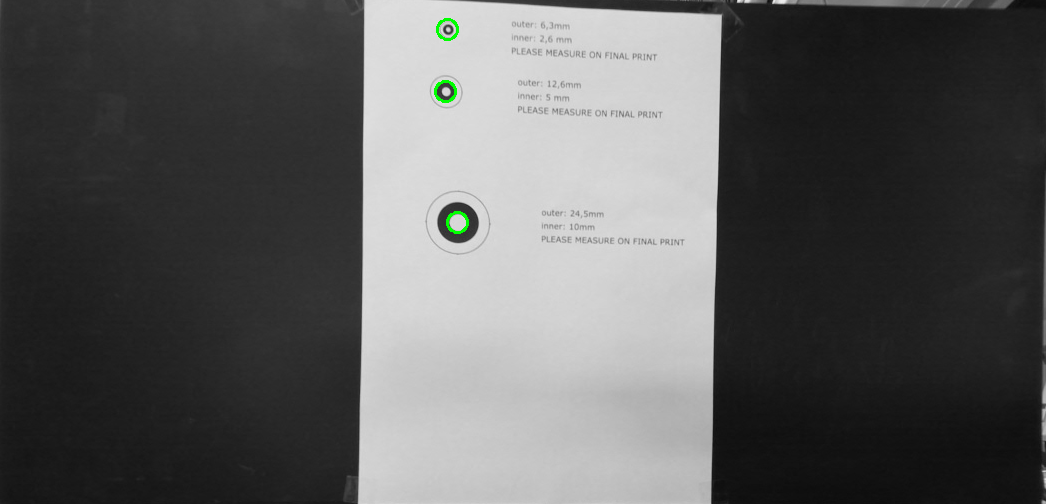
\includegraphics[width=\linewidth]{bilder/project/720p400mm.png}
        \caption{720p 400mm}\label{fig:720p400mm}
    \end{subfigure}
    \begin{subfigure}[b]{.45\linewidth}
        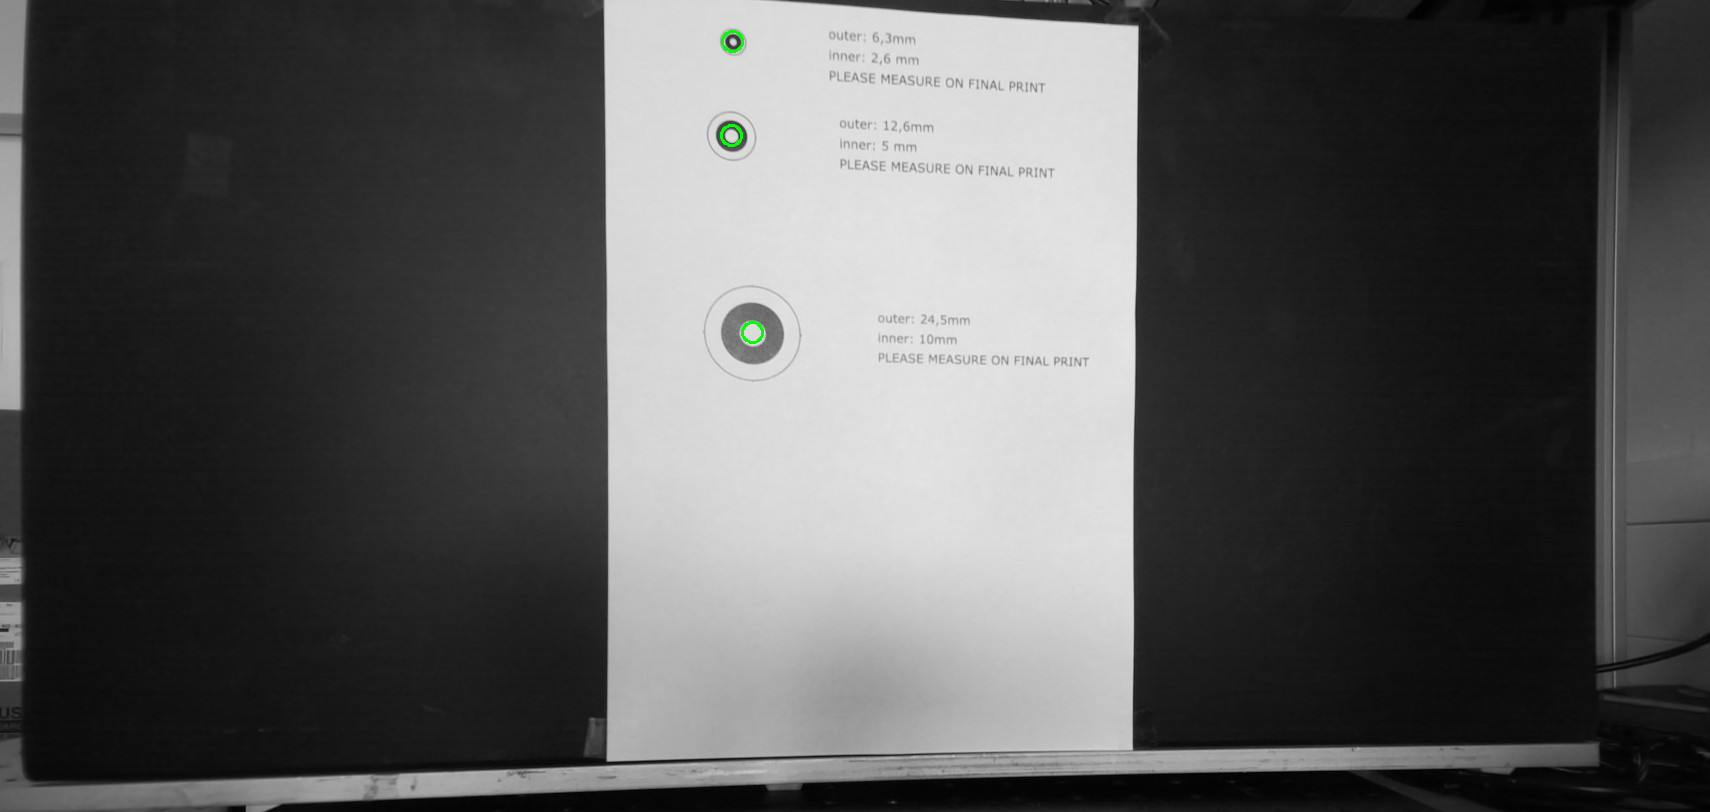
\includegraphics[width=\linewidth]{bilder/project/1080p400mm.png}
        \caption{1080p 400mm}\label{fig:1080p400mm}
    \end{subfigure}


    \begin{subfigure}[b]{.45\linewidth}
        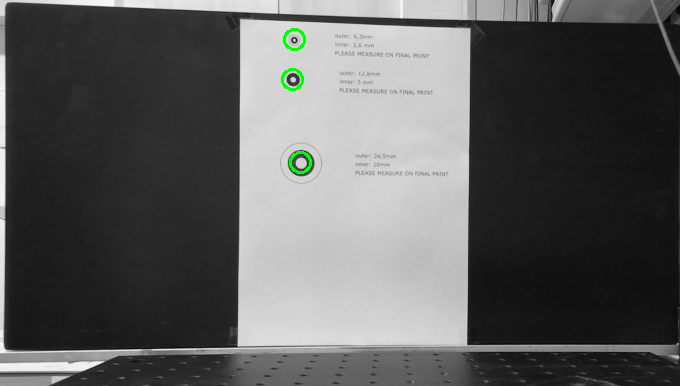
\includegraphics[width=\linewidth]{bilder/project/720p600mm.png}
        \caption{720p 600mm}\label{fig:720p600mm}
    \end{subfigure}
    \begin{subfigure}[b]{.45\linewidth}
        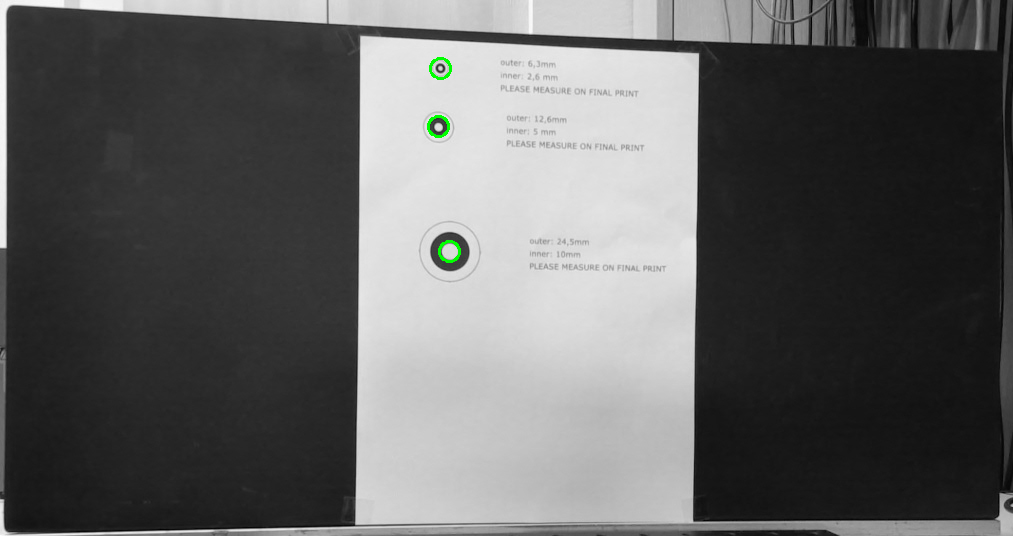
\includegraphics[width=\linewidth]{bilder/project/1080p600mm.png}
        \caption{1080p 600mm}\label{fig:1080p600mm}
    \end{subfigure}


    \begin{subfigure}[b]{.45\linewidth}
        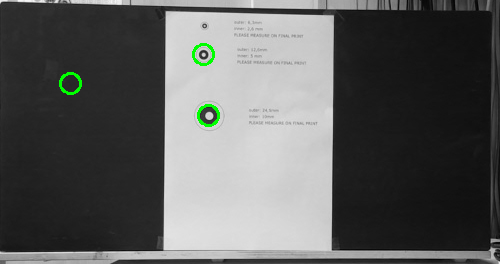
\includegraphics[width=\linewidth]{bilder/project/720p800mm.png}
        \caption{720p 800mm}\label{fig:720p800mm}
    \end{subfigure}
    \begin{subfigure}[b]{.45\linewidth}
        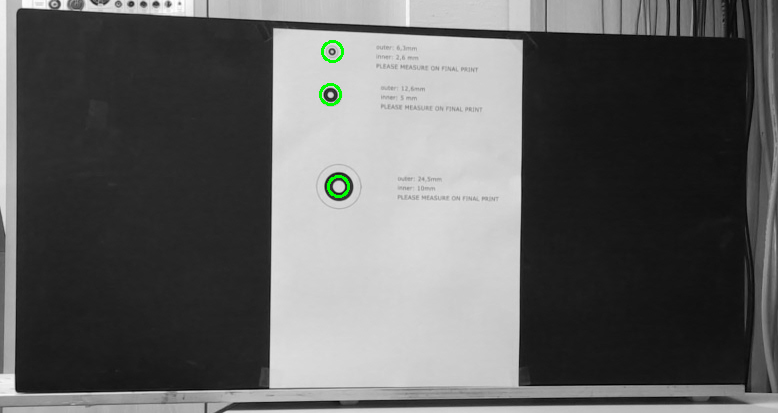
\includegraphics[width=\linewidth]{bilder/project/1080p800mm.png}
        \caption{1080p 800mm}\label{fig:1080p800mm}
    \end{subfigure}


    \begin{subfigure}[b]{.45\linewidth}
        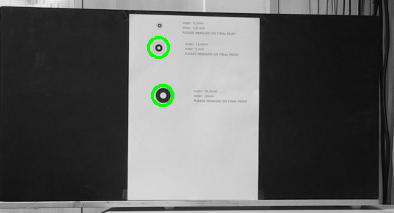
\includegraphics[width=\linewidth]{bilder/project/720p1000mm.png}
        \caption{720p 1000mm}\label{fig:720p1000mm}
    \end{subfigure}
    \begin{subfigure}[b]{.45\linewidth}
        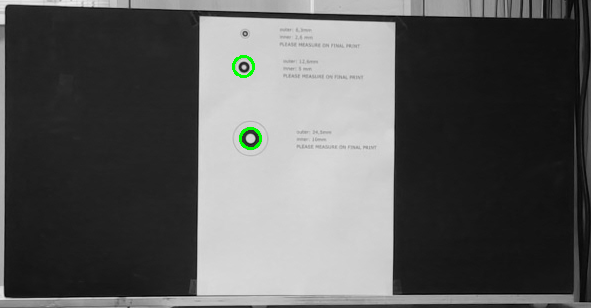
\includegraphics[width=\linewidth]{bilder/project/1080p1000mm.png}
        \caption{1080p 1000mm}\label{fig:1080p1000mm}
    \end{subfigure}
    \caption{Detection results of WHYCon marker at different distances and different resolutions}
    \label{fig:detection_results}
\end{figure}


\section{Tracking Performance}